
%\documentclass[tikz,convert={convertexe={magick.exe}}]{standalone}
\documentclass[tikz,convert]{standalone}
\usetikzlibrary{snakes}

\begin{document}
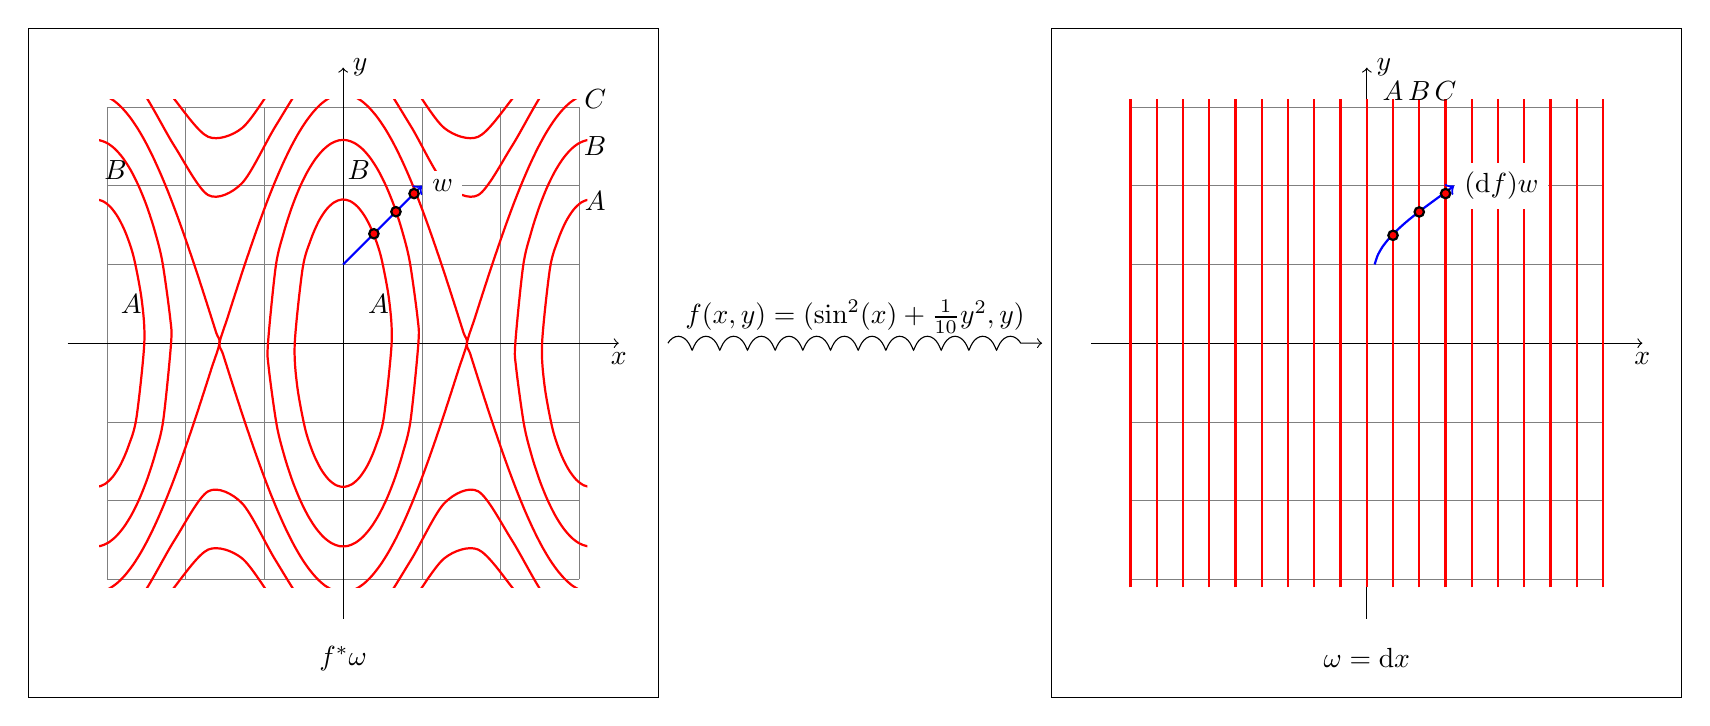
\begin{tikzpicture}

\tikzstyle atom=[circle, draw, inner sep=1.2pt, fill=red, thick]

\begin{scope}

\foreach \x in {-3,-2,...,3}
\draw[style=help lines, very thin] (\x,-3) -- (\x,3);
\foreach \y in {-3,-2,...,3}
\draw[style=help lines, very thin] (-3,\y) -- (3,\y);

\draw[->] (-3.5,0)--(3.5,0) node[below] {$x$};
\draw[->] (0,-3.5)--(0,3.5) node[right] {$y$};

\node (P) at (4,0) {};

\draw (-4,-4.5) rectangle (4,4);
\node at (0,-4) {$f^* \omega$};

\begin{scope}
\clip (-3.1,-3.1) rectangle (3.1,3.1);

\draw[red, thick] plot[smooth cycle] coordinates{(-0.615,0.000) (-0.515,0.950) (-0.415,1.305) (-0.315,1.540) (-0.215,1.696) (-0.115,1.789) (-0.015,1.825) (0.085,1.806) (0.185,1.731) (0.285,1.595) (0.385,1.388) (0.485,1.079) (0.585,0.537) (0.615,0.000) (0.515,-0.950) (0.415,-1.305) (0.315,-1.540) (0.215,-1.696) (0.115,-1.789) (0.015,-1.825) (-0.085,-1.806) (-0.185,-1.731) (-0.285,-1.595) (-0.385,-1.388) (-0.485,-1.079) (-0.585,-0.537)}; 
\draw[red, thick] plot[smooth cycle] coordinates{(2.526,0.000) (2.626,0.950) (2.726,1.305) (2.826,1.540) (2.926,1.696) (3.026,1.789) (3.126,1.825) (3.226,1.806) (3.326,1.731) (3.426,1.595) (3.526,1.388) (3.626,1.079) (3.726,0.537) (3.757,0.000) (3.657,-0.950) (3.557,-1.305) (3.457,-1.540) (3.357,-1.696) (3.257,-1.789) (3.157,-1.825) (3.057,-1.806) (2.957,-1.731) (2.857,-1.595) (2.757,-1.388) (2.657,-1.079) (2.557,-0.537)}; 
\draw[red, thick] plot[smooth cycle] coordinates{(-3.757,0.000) (-3.657,0.950) (-3.557,1.305) (-3.457,1.540) (-3.357,1.696) (-3.257,1.789) (-3.157,1.825) (-3.057,1.806) (-2.957,1.731) (-2.857,1.595) (-2.757,1.388) (-2.657,1.079) (-2.557,0.537) (-2.526,0.000) (-2.626,-0.950) (-2.726,-1.305) (-2.826,-1.540) (-2.926,-1.696) (-3.026,-1.789) (-3.126,-1.825) (-3.226,-1.806) (-3.326,-1.731) (-3.426,-1.595) (-3.526,-1.388) (-3.626,-1.079) (-3.726,-0.537)}; 
\draw[red, thick] plot[smooth cycle] coordinates{(-0.955,0.000) (-0.855,0.985) (-0.755,1.403) (-0.655,1.718) (-0.555,1.972) (-0.455,2.176) (-0.355,2.336) (-0.255,2.455) (-0.155,2.535) (-0.055,2.576) (0.045,2.578) (0.145,2.541) (0.245,2.466) (0.345,2.351) (0.445,2.195) (0.545,1.995) (0.645,1.748) (0.745,1.440) (0.845,1.037) (0.945,0.317) (0.955,0.000) (0.855,-0.985) (0.755,-1.403) (0.655,-1.718) (0.555,-1.972) (0.455,-2.176) (0.355,-2.336) (0.255,-2.455) (0.155,-2.535) (0.055,-2.576) (-0.045,-2.578) (-0.145,-2.541) (-0.245,-2.466) (-0.345,-2.351) (-0.445,-2.195) (-0.545,-1.995) (-0.645,-1.748) (-0.745,-1.440) (-0.845,-1.037) (-0.945,-0.317)}; 
\draw[red, thick] plot[smooth cycle] coordinates{(2.186,0.000) (2.286,0.985) (2.386,1.403) (2.486,1.718) (2.586,1.972) (2.686,2.176) (2.786,2.336) (2.886,2.455) (2.986,2.535) (3.086,2.576) (3.186,2.578) (3.286,2.541) (3.386,2.466) (3.486,2.351) (3.586,2.195) (3.686,1.995) (3.786,1.748) (3.886,1.440) (3.986,1.037) (4.086,0.317) (4.097,0.000) (3.997,-0.985) (3.897,-1.403) (3.797,-1.718) (3.697,-1.972) (3.597,-2.176) (3.497,-2.336) (3.397,-2.455) (3.297,-2.535) (3.197,-2.576) (3.097,-2.578) (2.997,-2.541) (2.897,-2.466) (2.797,-2.351) (2.697,-2.195) (2.597,-1.995) (2.497,-1.748) (2.397,-1.440) (2.297,-1.037) (2.197,-0.317)}; 
\draw[red, thick] plot[smooth cycle] coordinates{(-4.097,0.000) (-3.997,0.985) (-3.897,1.403) (-3.797,1.718) (-3.697,1.972) (-3.597,2.176) (-3.497,2.336) (-3.397,2.455) (-3.297,2.535) (-3.197,2.576) (-3.097,2.578) (-2.997,2.541) (-2.897,2.466) (-2.797,2.351) (-2.697,2.195) (-2.597,1.995) (-2.497,1.748) (-2.397,1.440) (-2.297,1.037) (-2.197,0.317) (-2.186,0.000) (-2.286,-0.985) (-2.386,-1.403) (-2.486,-1.718) (-2.586,-1.972) (-2.686,-2.176) (-2.786,-2.336) (-2.886,-2.455) (-2.986,-2.535) (-3.086,-2.576) (-3.186,-2.578) (-3.286,-2.541) (-3.386,-2.466) (-3.486,-2.351) (-3.586,-2.195) (-3.686,-1.995) (-3.786,-1.748) (-3.886,-1.440) (-3.986,-1.037) (-4.086,-0.317)}; 
\draw[red, thick] plot[smooth cycle] coordinates{(-1.571,0.000) (-1.471,0.316) (-1.371,0.628) (-1.271,0.935) (-1.171,1.231) (-1.071,1.516) (-0.971,1.786) (-0.871,2.037) (-0.771,2.268) (-0.671,2.477) (-0.571,2.661) (-0.471,2.818) (-0.371,2.947) (-0.271,3.047) (-0.171,3.116) (-0.071,3.154) (0.029,3.161) (0.129,3.136) (0.229,3.080) (0.329,2.992) (0.429,2.875) (0.529,2.730) (0.629,2.557) (0.729,2.358) (0.829,2.136) (0.929,1.893) (1.029,1.630) (1.129,1.351) (1.229,1.059) (1.329,0.757) (1.429,0.446) (1.529,0.131) (1.571,0.000) (1.471,-0.316) (1.371,-0.628) (1.271,-0.935) (1.171,-1.231) (1.071,-1.516) (0.971,-1.786) (0.871,-2.037) (0.771,-2.268) (0.671,-2.477) (0.571,-2.661) (0.471,-2.818) (0.371,-2.947) (0.271,-3.047) (0.171,-3.116) (0.071,-3.154) (-0.029,-3.161) (-0.129,-3.136) (-0.229,-3.080) (-0.329,-2.992) (-0.429,-2.875) (-0.529,-2.730) (-0.629,-2.557) (-0.729,-2.358) (-0.829,-2.136) (-0.929,-1.893) (-1.029,-1.630) (-1.129,-1.351) (-1.229,-1.059) (-1.329,-0.757) (-1.429,-0.446) (-1.529,-0.131)}; 
\draw[red, thick] plot[smooth cycle] coordinates{(1.571,0.000) (1.671,0.316) (1.771,0.628) (1.871,0.935) (1.971,1.231) (2.071,1.516) (2.171,1.786) (2.271,2.037) (2.371,2.268) (2.471,2.477) (2.571,2.661) (2.671,2.818) (2.771,2.947) (2.871,3.047) (2.971,3.116) (3.071,3.154) (3.171,3.161) (3.271,3.136) (3.371,3.080) (3.471,2.992) (3.571,2.875) (3.671,2.730) (3.771,2.557) (3.871,2.358) (3.971,2.136) (4.071,1.893) (4.171,1.630) (4.271,1.351) (4.371,1.059) (4.471,0.757) (4.571,0.446) (4.671,0.131) (4.712,0.000) (4.612,-0.316) (4.512,-0.628) (4.412,-0.935) (4.312,-1.231) (4.212,-1.516) (4.112,-1.786) (4.012,-2.037) (3.912,-2.268) (3.812,-2.477) (3.712,-2.661) (3.612,-2.818) (3.512,-2.947) (3.412,-3.047) (3.312,-3.116) (3.212,-3.154) (3.112,-3.161) (3.012,-3.136) (2.912,-3.080) (2.812,-2.992) (2.712,-2.875) (2.612,-2.730) (2.512,-2.557) (2.412,-2.358) (2.312,-2.136) (2.212,-1.893) (2.112,-1.630) (2.012,-1.351) (1.912,-1.059) (1.812,-0.757) (1.712,-0.446) (1.612,-0.131)}; 
\draw[red, thick] plot[smooth cycle] coordinates{(-4.712,0.000) (-4.612,0.316) (-4.512,0.628) (-4.412,0.935) (-4.312,1.231) (-4.212,1.516) (-4.112,1.786) (-4.012,2.037) (-3.912,2.268) (-3.812,2.477) (-3.712,2.661) (-3.612,2.818) (-3.512,2.947) (-3.412,3.047) (-3.312,3.116) (-3.212,3.154) (-3.112,3.161) (-3.012,3.136) (-2.912,3.080) (-2.812,2.992) (-2.712,2.875) (-2.612,2.730) (-2.512,2.557) (-2.412,2.358) (-2.312,2.136) (-2.212,1.893) (-2.112,1.630) (-2.012,1.351) (-1.912,1.059) (-1.812,0.757) (-1.712,0.446) (-1.612,0.131) (-1.571,0.000) (-1.671,-0.316) (-1.771,-0.628) (-1.871,-0.935) (-1.971,-1.231) (-2.071,-1.516) (-2.171,-1.786) (-2.271,-2.037) (-2.371,-2.268) (-2.471,-2.477) (-2.571,-2.661) (-2.671,-2.818) (-2.771,-2.947) (-2.871,-3.047) (-2.971,-3.116) (-3.071,-3.154) (-3.171,-3.161) (-3.271,-3.136) (-3.371,-3.080) (-3.471,-2.992) (-3.571,-2.875) (-3.671,-2.730) (-3.771,-2.557) (-3.871,-2.358) (-3.971,-2.136) (-4.071,-1.893) (-4.171,-1.630) (-4.271,-1.351) (-4.371,-1.059) (-4.471,-0.757) (-4.571,-0.446) (-4.671,-0.131)}; 
\draw[red, thick] plot[smooth] coordinates{(-3.000,3.624) (-2.571,3.228) (-2.143,2.503) (-1.714,1.881) (-1.286,2.031) (-0.857,2.760) (-0.429,3.407) (0.000,3.651) (0.429,3.407) (0.857,2.760) (1.286,2.031) (1.714,1.881) (2.143,2.503) (2.571,3.228) (3.000,3.624)}; 
\draw[red, thick] plot[smooth] coordinates{(-3.000,-3.624) (-2.571,-3.228) (-2.143,-2.503) (-1.714,-1.881) (-1.286,-2.031) (-0.857,-2.760) (-0.429,-3.407) (0.000,-3.651) (0.429,-3.407) (0.857,-2.760) (1.286,-2.031) (1.714,-1.881) (2.143,-2.503) (2.571,-3.228) (3.000,-3.624)}; 
\draw[red, thick] plot[smooth] coordinates{(-3.000,4.058) (-2.571,3.709) (-2.143,3.098) (-1.714,2.621) (-1.286,2.731) (-0.857,3.309) (-0.429,3.865) (0.000,4.082) (0.429,3.865) (0.857,3.309) (1.286,2.731) (1.714,2.621) (2.143,3.098) (2.571,3.709) (3.000,4.058)}; 
\draw[red, thick] plot[smooth] coordinates{(-3.000,-4.058) (-2.571,-3.709) (-2.143,-3.098) (-1.714,-2.621) (-1.286,-2.731) (-0.857,-3.309) (-0.429,-3.865) (0.000,-4.082) (0.429,-3.865) (0.857,-3.309) (1.286,-2.731) (1.714,-2.621) (2.143,-3.098) (2.571,-3.709) (3.000,-4.058)};

\end{scope}

\node at (.45,.5) {$A$};
\node at (.2,2.2) {$B$};
\node at (.45-pi,.5) {$A$};
\node at (.25-pi,2.2) {$B$};
\node at (3.2, 1.8) {$A$};
\node at (3.2, 2.5) {$B$};
\node at (3.2, 3.1) {$C$};


\draw[thick, blue, ->] (0,1)--(1,2) node[right,black,fill=white] {$w$};

\node[atom] at (.39,1.39) {};
\node[atom] at (.67,1.67) {};
\node[atom] at (.9,1.9) {};

\end{scope}

\begin{scope}[xshift=13cm]

\foreach \y in {-3,-2,...,3}
\draw[style=help lines, very thin] (-3,\y) -- (3,\y);

\draw[->] (-3.5,0)--(3.5,0) node[below] {$x$};
\draw[->] (0,-3.5)--(0,3.5) node[right] {$y$};

\node (Q) at (-4,0) {};

\draw (-4,-4.5) rectangle (4,4);
\node at (0,-4) {$\omega = \mathrm{d} x$};

\foreach \x in {-3,-2.66667,...,3}
\draw[red, thick] (\x,-3.1) -- (\x,3.1);

\node at (.333, 3.2) {$A$};
\node at (.666, 3.2) {$B$};
\node at (1, 3.2) {$C$};

\draw[thick,blue,->] plot[smooth] coordinates{(0.100,1.000) (0.136,1.111) (0.198,1.222) (0.285,1.333) (0.394,1.444) (0.520,1.556) (0.660,1.667) (0.808,1.778) (0.960,1.889) (1.108,2.000)} node[right,black,fill=white] {$(\mathrm{d}f)w$};

\node[atom] at (0.333,1.37) {};
\node[atom] at (0.666,1.667) {};
\node[atom] at (1,1.9) {};

\end{scope}


\draw[snake=coil, ->] (P) -- (Q) node[midway, above] {$f(x,y) = (\sin^2(x) + \frac1{10} y^2, y)$};

\end{tikzpicture}
\end{document}